% 07-references.tex - Section 7: References

\chapter{References}
\label{sec:references}

\section{Reference Documents}

\begin{enumerate}
    \item MCS Common ICD --- Monitor and Control System Common Interface Control Document

    \item DP ICD --- Digital Processor Interface Control Document (legacy system reference)

    \item Draft ADP ICD --- Draft version of the Advanced Digital Processor Interface Control Document

    \item ASP ICD --- Analog Signal Processor Interface Control Document

    \item LWA Station Architecture Document

    \item \label{ref:sievers-pfb} J.~Sievers, ``Inverting a Polyphase Filter Bank,'' unpublished note, 2022.  Distributed via the CASPER mailing list.  Reference implementation at \texttt{https://github.com/dcxSt/pfb-mod}.

\end{enumerate}

\section{Hardware References}

\begin{itemize}
    \item Xilinx ZCU102 Evaluation Kit User Guide (UG1182)
    \item Xilinx Zynq UltraScale+ MPSoC Data Sheet (DS891)
\end{itemize}

\section{Software Components}

The following software components implement the NDP system.  Table~\ref{tab:software-modules} lists the key modules.

\begin{table}[htbp]
    \centering
    \caption{NDP Software Modules}
    \label{tab:software-modules}
    \begin{tabular}{lp{8cm}}
        \toprule
        \textbf{Module} & \textbf{Description} \\
        \midrule
        \texttt{ndp\_control.py} & Main NDP control daemon; MCS command interface \\
        \texttt{ndp/Ndp.py} & Core NDP functions; command processing \\
        \texttt{ndp/NdpCommon.py} & Constants and fixed parameters \\
        \texttt{ndp/MCS2.py} & MCS message protocol implementation \\
        \texttt{ndp\_drx.py} & X-engine beamformer and correlator pipeline \\
        \texttt{ndp\_tengine.py} & T-engine pipeline (frequency to time domain) \\
        \texttt{lwa\_f} & F-engine control library (ZCU102 and SNAP2) \\
        \bottomrule
    \end{tabular}
\end{table}

\section{Pipeline Blocks}

The X-engine and T-engine processing pipelines are implemented as sequences of processing blocks defined in \texttt{ndp\_drx.py} and \texttt{ndp\_tengine.py}.  Table~\ref{tab:xengine-blocks} lists the X-engine blocks and Table~\ref{tab:tengine-blocks} lists the T-engine blocks.  Figures~\ref{fig:xengine-pipeline} and~\ref{fig:tengine-pipeline} show the corresponding Bifrost dataflow graphs, including the ring buffer data types between stages and CPU core assignments.

\begin{table}[htbp]
    \centering
    \caption{X-engine Pipeline Blocks (\texttt{ndp\_drx.py})}
    \label{tab:xengine-blocks}
    \begin{tabular}{lp{8cm}}
        \toprule
        \textbf{Block} & \textbf{Description} \\
        \midrule
        \texttt{CaptureOp} & F-engine packet capture and assembly \\
        \texttt{BufferCopyOp} & Ring buffer copy between pipeline stages \\
        \texttt{GPUCopyOp} & Host-to-GPU data transfer \\
        \texttt{PowerLineFlaggerOp} & Power line interference flagging (Appendix~\ref{app:powerline}) \\
        \texttt{BeamformerOp} & GPU beamformer (delay, gain, and sum) \\
        \texttt{CorrelatorOp} & GPU correlator (full visibility matrix) \\
        \texttt{TriggeredDumpOp} & TBT triggered spectra dump \\
        \texttt{StreamingOp} & TBS continuous spectra streaming \\
        \texttt{RetransmitOp} & Beamformed data retransmission to T-engines \\
        \texttt{PacketizeOp} & COR output packetization \\
        \bottomrule
    \end{tabular}
\end{table}

\begin{figure}[htbp]
    \centering
    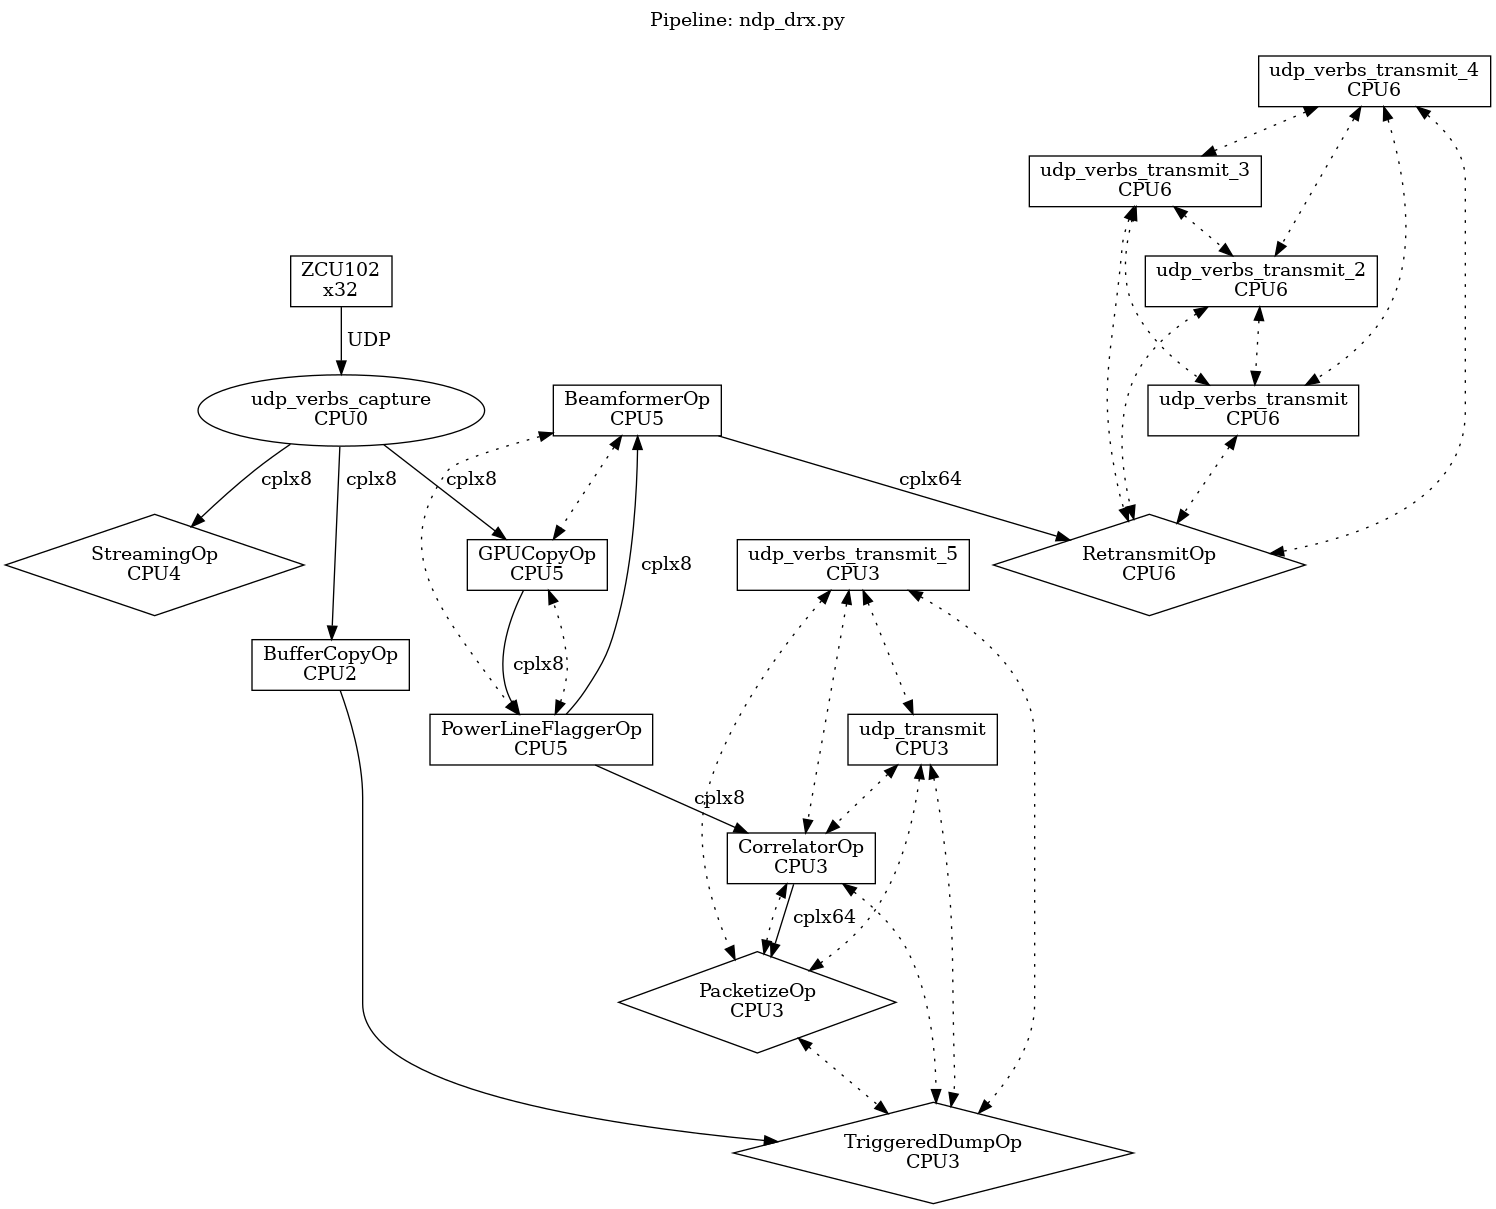
\includegraphics[width=\textwidth]{figures/xengine.png}
    \caption{X-engine Bifrost pipeline dataflow graph.  Solid lines indicate ring buffer connections with data types labeled (cplx8/cplx64).  Dotted lines indicate sequence callback connections.  Node shapes follow Bifrost conventions: ellipses for capture blocks, rectangles for processing blocks, and diamonds for output/transmit blocks.}
    \label{fig:xengine-pipeline}
\end{figure}

\begin{table}[htbp]
    \centering
    \caption{T-engine Pipeline Blocks (\texttt{ndp\_tengine.py})}
    \label{tab:tengine-blocks}
    \begin{tabular}{lp{8cm}}
        \toprule
        \textbf{Block} & \textbf{Description} \\
        \midrule
        \texttt{CaptureOp} & Beamformed data capture from X-engines \\
        \texttt{GPUCopyOp} & Host-to-GPU data transfer \\
        \texttt{ReChannelizerOp} & Inverse polyphase filter bank (Appendix~\ref{app:pfbinverse}) \\
        \texttt{TEngineOp} & Frequency-to-time domain conversion \\
        \texttt{PacketizeOp} & DRX/DRX8 output packetization \\
        \bottomrule
    \end{tabular}
\end{table}

\begin{figure}[htbp]
    \centering
    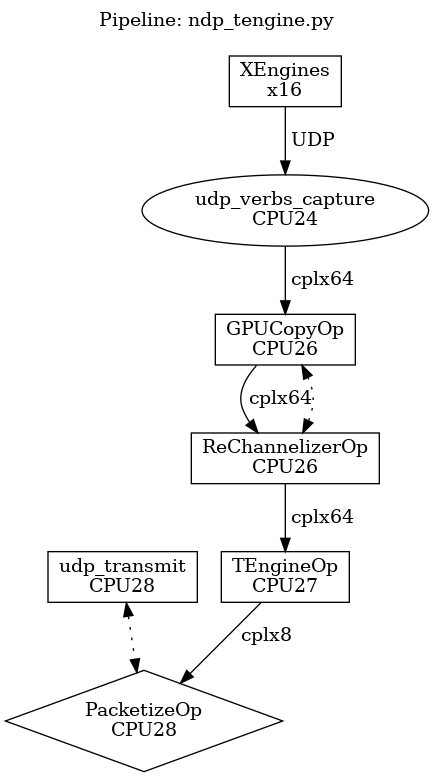
\includegraphics[width=0.45\textwidth]{figures/tengine.png}
    \caption{T-engine Bifrost pipeline dataflow graph.  The pipeline is primarily linear, converting frequency-domain beamformed data (cplx64) to time-domain output (cplx8) via the inverse polyphase filter bank and T-engine blocks.}
    \label{fig:tengine-pipeline}
\end{figure}

\section{Configuration}
\label{sec:configuration}

NDP configuration is stored in JSON format in site-specific files
(\texttt{ndp\_config.json.\textit{site}}).  The top-level keys and their
nested structure are described below.

\subsection{Global Parameters}

Three top-level scalar parameters control NDP daemon timing (Table~\ref{tab:config-global}).

\begin{table}[htbp]
    \centering
    \caption{Top-level Configuration Parameters}
    \label{tab:config-global}
    \begin{tabular}{llp{7cm}}
        \toprule
        \textbf{Key} & \textbf{Type} & \textbf{Description} \\
        \midrule
        \texttt{shutdown\_timeout}  & float & Graceful shutdown timeout (seconds) \\
        \texttt{monitor\_interval}  & float & System monitoring interval (seconds) \\
        \texttt{failsafe\_interval} & float & Failsafe check interval (seconds) \\
        \bottomrule
    \end{tabular}
\end{table}

\subsection{\texttt{mcs} --- MCS Communication}

The \texttt{mcs} object configures the UDP interface between NDP and MCS, split into headnode and server sub-objects (Table~\ref{tab:config-mcs}).

\begin{table}[htbp]
    \centering
    \caption{\texttt{mcs} Configuration Parameters}
    \label{tab:config-mcs}
    \begin{tabular}{llp{7cm}}
        \toprule
        \textbf{Key} & \textbf{Type} & \textbf{Description} \\
        \midrule
        \multicolumn{3}{l}{\textit{\texttt{mcs.headnode}}} \\
        \quad\texttt{local\_host}       & string & Bind address for receiving MCS commands \\
        \quad\texttt{local\_port}       & int    & UDP port for receiving MCS commands \\
        \quad\texttt{remote\_host}      & string & MCS host address for sending responses \\
        \quad\texttt{remote\_host\_TEST}& string & Alternate MCS host for testing \\
        \quad\texttt{remote\_port}      & int    & UDP port for sending MCS responses \\
        \midrule
        \multicolumn{3}{l}{\textit{\texttt{mcs.server}}} \\
        \quad\texttt{local\_host}       & string & Bind address for server-side MCS interface \\
        \quad\texttt{local\_port}       & int    & UDP port for server-side MCS interface \\
        \bottomrule
    \end{tabular}
\end{table}

\subsection{\texttt{host} --- System Hostnames}

The \texttt{host} object maps logical roles to network hostnames (Table~\ref{tab:config-host}).

\begin{table}[htbp]
    \centering
    \caption{\texttt{host} Configuration Parameters}
    \label{tab:config-host}
    \begin{tabular}{llp{7cm}}
        \toprule
        \textbf{Key} & \textbf{Type} & \textbf{Description} \\
        \midrule
        \texttt{servers}      & array of string & X-engine server hostnames \\
        \texttt{fpgas}        & array of string & F-engine board hostnames \\
        \texttt{servers-data} & array of string & Data network interface hostnames (two per server) \\
        \texttt{tengines}     & array of string & T-engine host identifiers \\
        \bottomrule
    \end{tabular}
\end{table}

\subsection{\texttt{ipmi} --- IPMI Credentials}

The \texttt{ipmi} object provides credentials for out-of-band server management (Table~\ref{tab:config-ipmi}).

\begin{table}[htbp]
    \centering
    \caption{\texttt{ipmi} Configuration Parameters}
    \label{tab:config-ipmi}
    \begin{tabular}{llp{7cm}}
        \toprule
        \textbf{Key} & \textbf{Type} & \textbf{Description} \\
        \midrule
        \texttt{username} & string & IPMI username \\
        \texttt{password} & string & IPMI password \\
        \bottomrule
    \end{tabular}
\end{table}

\subsection{\texttt{fpga} --- F-engine Configuration}

The \texttt{fpga} object configures the F-engine boards, including FPGA firmware, filter bank settings, and temperature thresholds (Table~\ref{tab:config-fpga}).

\begin{table}[htbp]
    \centering
    \caption{\texttt{fpga} Configuration Parameters}
    \label{tab:config-fpga}
    \begin{tabular}{llp{7cm}}
        \toprule
        \textbf{Key} & \textbf{Type} & \textbf{Description} \\
        \midrule
        \texttt{username}             & string         & SSH username for F-engine boards (ZCU102 only) \\
        \texttt{password}             & string         & SSH password for F-engine boards (ZCU102 only) \\
        \texttt{data\_ip\_base}       & string         & Base IP address for F-engine data interfaces \\
        \texttt{data\_port\_base}     & int            & Base UDP port for F-engine data output \\
        \texttt{firmware}             & string         & Path to FPGA firmware file (\texttt{.fpg}) \\
        \texttt{max\_program\_attempts} & int          & Maximum FPGA programming retries \\
        \texttt{fft\_shift}           & int            & FFT shift schedule for the polyphase filter bank \\
        \texttt{equalizer\_coeffs}    & string         & Path to equalizer coefficient file \\
        \texttt{bypass\_pfb}          & bool           & Bypass the polyphase filter bank \\
        \texttt{nchan\_packet}        & int            & Number of frequency channels per output packet \\
        \texttt{temperatures}         & array of string & IPMI temperature sensor names \\
        \texttt{temperature\_warning} & float          & Warning temperature threshold (\si{\degreeCelsius}) \\
        \texttt{temperature\_shutdown}& float          & Shutdown temperature threshold (\si{\degreeCelsius}) \\
        \texttt{temperature\_scram}   & float          & Emergency shutdown threshold (\si{\degreeCelsius}) \\
        \bottomrule
    \end{tabular}
\end{table}

\subsection{\texttt{server} --- X-engine Server Configuration}

The \texttt{server} object configures the X-engine GPU servers, including data network interfaces, resource monitoring, and temperature thresholds (Table~\ref{tab:config-server}).

\begin{table}[htbp]
    \centering
    \caption{\texttt{server} Configuration Parameters}
    \label{tab:config-server}
    \begin{tabular}{llp{7cm}}
        \toprule
        \textbf{Key} & \textbf{Type} & \textbf{Description} \\
        \midrule
        \texttt{username}             & string         & SSH/management username \\
        \texttt{password}             & string         & SSH/management password \\
        \texttt{cpu\_ids}             & array of int   & CPU socket IDs to monitor \\
        \texttt{gpu\_ids}             & array of int   & GPU device IDs to monitor \\
        \texttt{disk\_ids}            & array of string & Disk mount points to monitor \\
        \texttt{data\_ports}          & array of int   & UDP data reception ports (one per server) \\
        \texttt{data\_ifaces}         & array of string & Network interface names for data reception \\
        \texttt{startup\_timeout}     & int            & Server startup timeout (seconds) \\
        \texttt{temperatures}         & array of string & IPMI temperature sensor names \\
        \texttt{temperature\_warning} & float          & Warning temperature threshold (\si{\degreeCelsius}) \\
        \texttt{temperature\_shutdown}& float          & Shutdown temperature threshold (\si{\degreeCelsius}) \\
        \texttt{temperature\_scram}   & float          & Emergency shutdown threshold (\si{\degreeCelsius}) \\
        \bottomrule
    \end{tabular}
\end{table}

\subsection{\texttt{drx} --- X-engine Pipeline Configuration}

The \texttt{drx} key is an array of objects, one per X-engine pipeline instance.
Each pipeline processes a contiguous range of frequency channels (Table~\ref{tab:config-drx}).

\begin{table}[htbp]
    \centering
    \caption{\texttt{drx[\textit{i}]} Configuration Parameters}
    \label{tab:config-drx}
    \begin{tabular}{llp{7cm}}
        \toprule
        \textbf{Key} & \textbf{Type} & \textbf{Description} \\
        \midrule
        \texttt{first\_channel}       & int          & First frequency channel index processed \\
        \texttt{capture\_bandwidth}   & float        & Capture bandwidth (Hz) \\
        \texttt{beam\_count}          & int          & Number of beams produced \\
        \texttt{pipeline\_idx}        & int          & Pipeline index on the host server \\
        \texttt{tengine\_idx}         & array of int & T-engine indices receiving beamformed data \\
        \texttt{tbx\_recorder\_idx}   & int          & Recorder index for TBT/TBS output \\
        \texttt{cor\_recorder\_idx}   & int          & Recorder index for correlator output \\
        \texttt{cpus}                 & array of int & CPU core IDs allocated to this pipeline \\
        \texttt{gpus}                 & array of int & GPU device IDs allocated to this pipeline \\
        \texttt{powerline\_flagger}   & bool         & Enable power line interference flagging \\
        \bottomrule
    \end{tabular}
\end{table}

\subsection{\texttt{tengine} --- T-engine Pipeline Configuration}

The \texttt{tengine} key is an array of objects, one per T-engine pipeline
instance (Table~\ref{tab:config-tengine}).

\begin{table}[htbp]
    \centering
    \caption{\texttt{tengine[\textit{i}]} Configuration Parameters}
    \label{tab:config-tengine}
    \begin{tabular}{llp{7cm}}
        \toprule
        \textbf{Key} & \textbf{Type} & \textbf{Description} \\
        \midrule
        \texttt{pipeline\_idx}  & int          & Pipeline index on the host server \\
        \texttt{recorder\_idx}  & int          & Recorder index for DRX output \\
        \texttt{cpus}           & array of int & CPU core IDs allocated to this pipeline \\
        \texttt{gpus}           & array of int & GPU device IDs allocated to this pipeline \\
        \texttt{pfb\_inverter}  & bool         & Enable inverse polyphase filter bank for DRX output \\
        \bottomrule
    \end{tabular}
\end{table}

\subsection{\texttt{recorder} --- Data Recorder Configuration}

The \texttt{recorder} key is an array of objects, one per data recorder.
Recorders are referenced by index from the \texttt{drx} and \texttt{tengine}
pipeline configurations (Table~\ref{tab:config-recorder}).

\begin{table}[htbp]
    \centering
    \caption{\texttt{recorder[\textit{i}]} Configuration Parameters}
    \label{tab:config-recorder}
    \begin{tabular}{llp{7cm}}
        \toprule
        \textbf{Key} & \textbf{Type} & \textbf{Description} \\
        \midrule
        \texttt{host}              & string & Recorder hostname or IP address \\
        \texttt{port}              & int    & UDP receive port on the recorder \\
        \texttt{max\_bytes\_per\_sec} & int & Maximum output data rate (bytes/sec) \\
        \bottomrule
    \end{tabular}
\end{table}

\subsection{\texttt{tbt} --- Transient Buffer Triggered Configuration}

The \texttt{tbt} object controls the transient buffer triggered capture ring buffer (Table~\ref{tab:config-tbt}).

\begin{table}[htbp]
    \centering
    \caption{\texttt{tbt} Configuration Parameters}
    \label{tab:config-tbt}
    \begin{tabular}{llp{7cm}}
        \toprule
        \textbf{Key} & \textbf{Type} & \textbf{Description} \\
        \midrule
        \texttt{buffer\_time\_sec} & float & TBT ring buffer duration (seconds) \\
        \bottomrule
    \end{tabular}
\end{table}

\subsection{\texttt{log} --- Logging Configuration}

The \texttt{log} object controls log file rotation, formatting, and output paths (Table~\ref{tab:config-log}).

\begin{table}[htbp]
    \centering
    \caption{\texttt{log} Configuration Parameters}
    \label{tab:config-log}
    \begin{tabular}{llp{7cm}}
        \toprule
        \textbf{Key} & \textbf{Type} & \textbf{Description} \\
        \midrule
        \texttt{days\_per\_file}  & int    & Log file rotation period (days) \\
        \texttt{max\_file\_count} & int    & Maximum number of retained log files \\
        \texttt{msg\_format}      & string & Python \texttt{logging} message format \\
        \texttt{stats\_format}    & string & Statistics log message format \\
        \texttt{date\_format}     & string & Date format string for log entries \\
        \midrule
        \multicolumn{3}{l}{\textit{\texttt{log.files}}} \\
        \quad\texttt{server\_temps} & string & Path to server temperature log file \\
        \quad\texttt{roach\_temps}  & string & Path to F-engine temperature log file \\
        \bottomrule
    \end{tabular}
\end{table}

\section{Source Code Repositories}

\begin{itemize}
    \item NDP Control Software: \texttt{ng\_digital\_processor}
    \item F-engine Control: \texttt{lwa\_f}
\end{itemize}
